\Transcb{yellow}{blue}{The Robertson-Walker metric}
\onecolumn
\begin{itemize}
\item Observation : All galaxies at large distances are moving away from us
\item[] Isotropic universe $\rightarrow$ All distant galaxies are moving away from each other
\item[$\ast$] Consequence : {\blue The universe is expanding !}
\item[] Comparison : Cooking of a pudding with raisins in it 
\item Expansion in an isotropic homogeneous universe 
\item[] Observer $B$ observes objects $A$ and $C$ at physical distances $d(t)$ as shown below
\item[] \begin{center}
        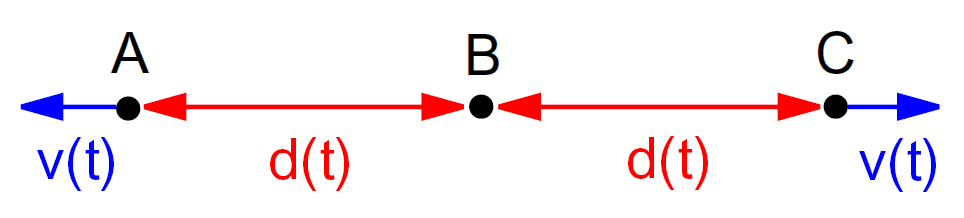
\includegraphics[keepaspectratio,width=10cm]{abc}
        \end{center}
\item[] Expansion as seen from $B$ : $A$ and $C$ move with equal speed $v(t)$ in opposite directions
\item[] Expansion as seen from $A$ : $B$ moves away with speed $v(t)$ and $C$ with speed $2v(t)$
\item[] Expansion as seen from $C$ : $B$ moves away with speed $v(t)$ and $A$ with speed $2v(t)$
\item[$\ast$] Consequently : {\blue $v(t)=H(t)d(t)$} where {\blue $H(t) \equiv$ Hubble parameter}
\item[] Using $v(t)=\dot{d}(t)$ we can write {\red $\dot{d}(t)=H(t)d(t)$}
\item[] {\blue Can we obtain an expression for the spatial evolution d(t) of the universe from this ?}
\end{itemize}

\Tr
\begin{itemize}
\item Starting expression for the space-time description of the universe : {\blue $\dot{d}(t)=H(t)d(t)$}
\item[] Solution to this differential equation : {\blue $d(t)=a(t)\chi$} with {\blue $\chi \equiv$ constant}
\item[$\ast$] Interpretation of this solution
\item[] At some time origin every object is given a {\blue fixed radial distance $\chi$}
\item[] Expansion is then described by the {\blue cosmic expansion factor $a(t)$} via $d(t)=a(t)\chi$
\item[] $\displaystyle \rightarrow \dot{d}(t)=\dot{a}(t)\chi=\frac{\dot{a}(t)}{a(t)}\,a(t)\chi
         =\frac{\dot{a}(t)}{a(t)}\,d(t) \Rightarrow {\blue H(t)=\frac{\dot{a}(t)}{a(t)}}$
\item[$\ast$] {\red All distances in the universe increase by the cosmic expansion factor $a(t)$}
\item The same procedure can be performed for coordinates
\item[] At some time origin every object is given a {\blue fixed comoving radial coordinate $\sigma$}
\item[] Expansion is then described via {\blue $r(t)=a(t)\sigma$}
\item[$\ast$] Description in {\blue comoving spherical coordinates $(\sigma,\theta,\varphi)$}
\item[] Always proper time $\d\tau$ on comoving spherical shell $\rightarrow$
        {\blue No time distortion in the metric}
\item[] This reference frame is at rest w.r.t. the average matter of the universe (i.e. CMBR)
\end{itemize}

\Tr
\begin{itemize}
\item Using {\blue $\d r=a(t)\d\sigma$} and using the arbitrary scale of $\sigma$ we can write
\item[] {\blue $\displaystyle K(t) \equiv \frac{k}{a^{2}(t)} \text{ with } k=
         \begin{cases}
         1 & \text{positive curvature (i.e. closed space)}\\
         0 & \text{no curvature (i.e. flat space)}\\
         -1 & \text{negative curvature (i.e. open space)}
         \end{cases}
        $}
\item[] the space-time metric for constant curvature in comoving coordinates becomes
\item[] \begin{center}
         {\red \shabox{$\displaystyle
         \d s^{2}=(c\,\d t)^{2}-a^{2}(t)\left[
         \frac{(\d\sigma)^{2}}{1-k\sigma^{2}}+\sigma^{2}(\d\theta)^{2}+\sigma^{2}\sin^{2}(\theta)(\d\varphi)^{2}
         \right]$}}
        \end{center}
\item[] which is called the {\blue Robertson-Walker metric}
\item Derived purely by symmetry arguments of 3D-space and extension to 4D space-time
\item Describes the universe in comoving coordinates
\item[] $\rightarrow$ The most natural reference frame : the one at rest w.r.t. the CMBR
\item[$\ast$] It is the only solution to Einstein's equations for a homogeneous and isotropic universe
\item[] {\blue Can we also obtain an expression for a(t) to make our description complete ?}
\end{itemize}
